\documentclass[onecolumn]{article}
%\usepackage{url}
%\usepackage{algorithmic}
\usepackage[a4paper]{geometry}
\usepackage{datetime}
\usepackage{hyperref}
\usepackage[margin=2em, font=small,labelfont=it]{caption}
\usepackage{graphicx}
\usepackage{mathpazo} % use palatino
\usepackage[scaled]{helvet} % helvetica
\usepackage{microtype}
\usepackage{amsmath}
\usepackage{subfigure}
\usepackage{listings}
\usepackage{float}
\usepackage{xcolor} %red, green, blue, yellow, cyan, magenta, black, white
\usepackage{graphicx}
\usepackage[font=small,labelfont=bf]{caption}
\renewcommand{\thefigure}{\arabic{section}.\arabic{figure}}
\graphicspath{ {pictures/} }
\definecolor{mygreen}{RGB}{28,172,0} % color values Red, Green, Blue
\definecolor{lightgray}{gray}{0.9}
\definecolor{mylilas}{RGB}{170,55,241}
\newcommand{\inlinecode}[2]{\colorbox{lightgray}{\lstinline[language=#1]$#2$}}


% Letterspacing macros
\newcommand{\spacecaps}[1]{\textls[200]{\MakeUppercase{#1}}}
\newcommand{\spacesc}[1]{\textls[50]{\textsc{\MakeLowercase{#1}}}}
\newcommand{\inline}[1]{\colorbox{lightgray}{\lstinline[basicstyle=\ttfamily\color{brown}]|#1|}}

\title{\spacecaps{Lab report: Lab 6 }\\
Taylor model – explicit method\\\normalsize \spacesc{Modeling of Physical Systems} }

\author{Patryk Gałczyński}
%\date{\today\\\currenttime}
\date{\today}


\begin{document}
\lstset{language=Matlab,%
    %basicstyle=\color{red},
    %breaklines=true,%
    morekeywords={matlab2tikz},
    keywordstyle=\color{blue},%
    morekeywords=[2]{1}, keywordstyle=[2]{\color{black}},
    identifierstyle=\color{black},%
    stringstyle=\color{mylilas},
    commentstyle=\color{mygreen},%
    showstringspaces=false,%without this there will be a symbol in the places where there is a space
    numbers=left,%
    numberstyle={\small \color{black}},% size of the numbers
    numbersep=9pt, % this defines how far the numbers are from the text
    emph=[1]{for,end,break},emphstyle=[1]\color{red}, %some words to emphasise
    %emph=[2]{word1,word2}, emphstyle=[2]{style},    
}

\maketitle


\section{Aim}
\large
The aim of this laboratory was to simulate, visualize and analyze simplified Taylor model of one dimensional river pollutants transportation process using "QUICKEST explicit method".


\section{Simulation description}
Pollutants transportation process can be modeled by following Taylor equation:
\begin{equation}
\frac{\partial c}{\partial t} + U \frac{\partial c}{\partial x} - D \frac{\partial ^ 2 c}{\partial x^2} = 0
\end{equation}
Such model requires to define boundary conditions as well as initial conditions:
\begin{enumerate}
	\item boundary condition - left side - $c(0,t) = 0$
    \item boundary condition - right side - $\frac{\partial c}{\partial x}(L,t) = 0$
    \item initial condition - $c(x, 0) = \begin{cases} 0 \quad \quad \quad \text{for} \quad x \neq x_i \\ \frac{m}{w \cdot d \cdot dx} \quad \text{for} \quad x = x_i \end{cases}$
\end{enumerate}
where:
\begin{itemize}
	\item c - tracer’s concentration function
    \item t - time variable
    \item U = $0.1 [\frac{m}{s}]$- advection coefficient
    \item x - displacement
    \item D = $0.01 [\frac{m^2}{s}]$ - dispersion coefficient
    \item L = $100 [m]$ - river length
    \item m = $1 [kg]$ - mass of injected tracer
    \item w = $5 [m]$ - river width
    \item d = $1 [m]$ - river depth
\end{itemize}

Given differential equation would be hard to model within matlab script, which is why numerical approach was chosen over the analytical one. In this case, explicit quickest method provides fairly easy formula to implement, and most importantly it provides iterative interface (next function value is being calculated based on previously calculated one). Following this approach, one can propose following formula:
\begin{multline}
{c_j}^{n+1} = {c^n_j} + [C_d(1 - C_a) - \frac{C_a}{6}(C_a^2 - 3C_a + 2)]{c^n_{j+1}} - [C_d(2 - 3C_a) - \frac{C_a}{2}(C_a^2 - 2C_a - 1)]{c^n_{j}}\\ +
[C_d(1 - 3C_a) - \frac{C_a}{2}(C_a^2 - C_a - 2)]{c^n_{j-1}} + 
[C_d C_a - \frac{C_a}{6}(C_a^2 - 1)]{c^n_{j-2}}
\end{multline}
where:
\begin{itemize}
    \item $C_a$ - advective Courant number
    \item $C_d$ - diffusive Courant number
\end{itemize}

\subsection{Quickest method implementation}
To realize provided algorithm, simple matlab script were developed:
\begin{lstlisting}[language=Matlab,frame=single,label={lst:autocorr},breaklines=true,caption={Matlab script for explicit taylor method}]
% define parameters
len     = 100;    % m
wid     = 5;      % m
dep     = 1;      % m

t       = 1000;   % s
dt      = 1;    % s
dx      = 1;    % m
nt      = t/dt;   % num
U       = 0.1;    % m/s  [advection coefficient ]
D       = 0.01;   % m2/s [dispersion coefficient] 
inject  = 10;     % m
measure = 90;     % m
tracer  = 1;      % kg

Ca = U * dt / dx;
Cd = D * dt / dx^2;
c = [];

% initial condition
for j = 1:(len/dx)
    if j*dx == inject
        c(1,j) = tracer/(dx*dep*wid);
    else
        c(1, j) = 0;
    end
end

% calculate in real time
for i = 1:(t/dt)
    for j = 3:(len/dx)-1
        c(i+1, j) = c(i, j) + ...
            (Cd*(1-Ca) - (Ca/6)*(Ca^2 - 3*Ca + 2))*c(i,j+1) - ...
            (Cd*(2 - 3*Ca) - (Ca/2)*(Ca^2 - 2*Ca - 1))*c(i,j) + ...
            (Cd*(1 - 3*Ca) - (Ca/2)*(Ca^2 - Ca - 2))*c(i,j-1) + ...
            (Cd*Ca + (Ca/6)*(Ca^2 - 1))*c(i,j-2);
    end
    
    % plot results
    subplot(2,1,1);
    plot(1:(len/dx), c(i,:));
    xlabel('t');
    ylabel('c(t)');
    xlim([0 100]);
    ylim([0 0.1]);
    subplot(2,1,2);
    plot(c(:,measure/dx));
    xlabel('x');
    ylabel('c(x)');
    drawnow;
    pause(0.1);
end
\end{lstlisting}
This script simulates, how 1kg of tracer is being moved by the river. At runtime, it produces constant animation, showing tracer spatial distribution over time and change of tracer at given point (measure point) over time.
Below, two pictures from different timestamps were shown:

\noindent\makebox[\textwidth]{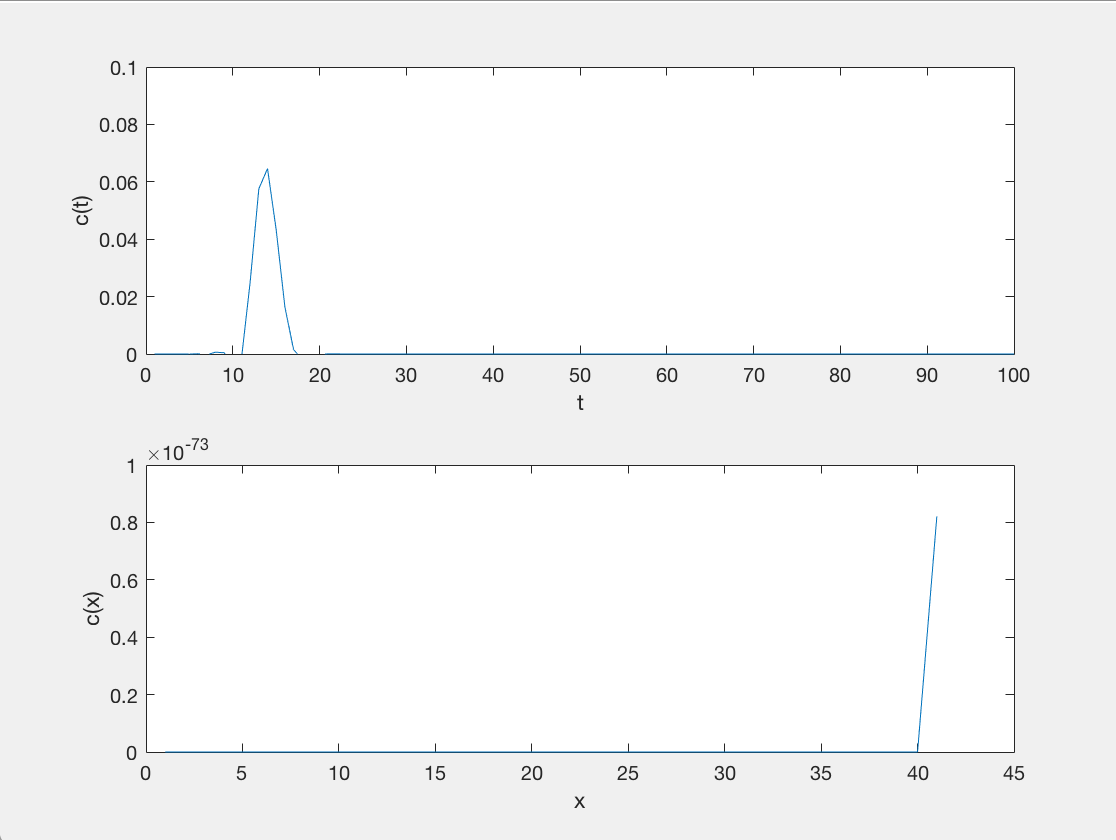
\includegraphics[scale=0.5]{s1}}
\noindent\makebox[\textwidth]{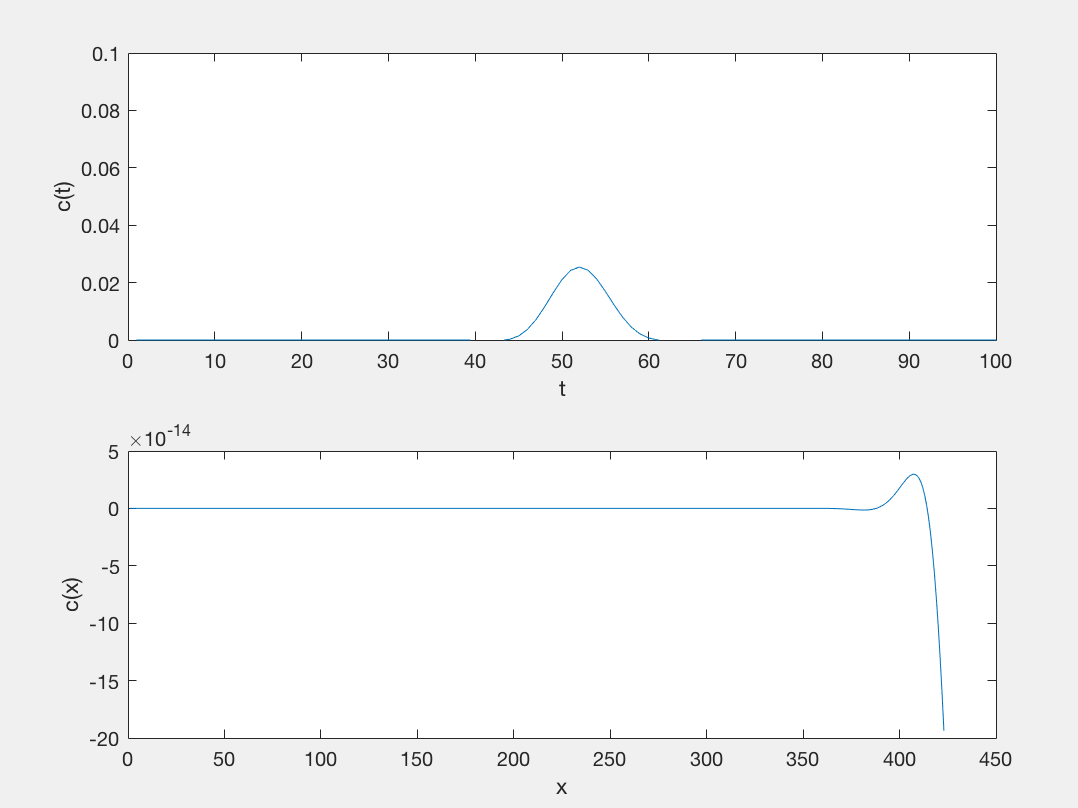
\includegraphics[scale=0.5]{s2}}

It is clearly visible that the "plateau" moves towards right over time, it makes sense as tracer flows within river. Also, as river and time flows, it is observable that amount of tracer at measure point variates in time (I guess it oscillates, sometime it increases, sometime it decreases).

\subsection{Numerical stability}
Due to numerical algorithm properties, there is a change that for given parameters, this numerical model will remain unstable. To check such behavior, it should be observable that for small change, one would see huge change in obtained results. For this purpose, various parameters were checked for such behavior.

\begin{enumerate}
	\item dx between 0.1m (left one) and 1m (right one) \\
    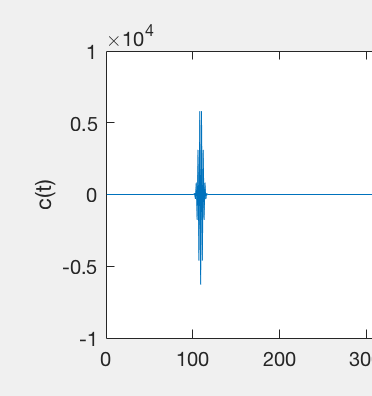
\includegraphics[scale=1]{dx01}
	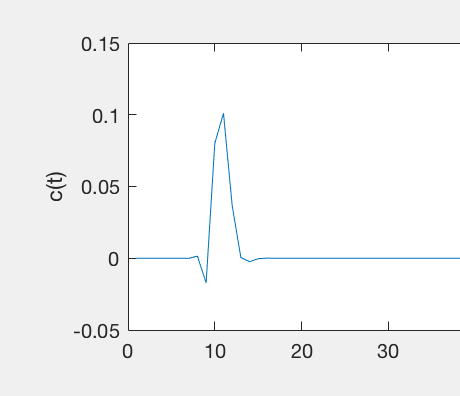
\includegraphics[scale=1]{dx1}
    
    \item dt between 15s (left one) and 16s (right one) \\
    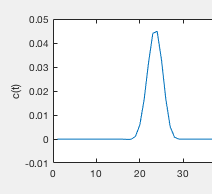
\includegraphics[scale=1]{dt15}
	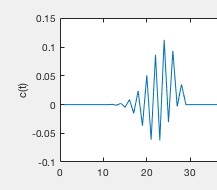
\includegraphics[scale=1]{dt16}
    
    \item Advection coefficient between 0.1 (left one) and 5 (right one) \\
    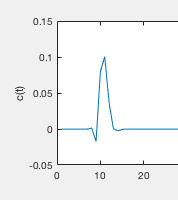
\includegraphics[scale=1]{u01}
	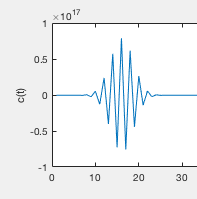
\includegraphics[scale=1]{u5}
    
    \item Dispersion coefficient between 0.5 (left one) and 0.6 (right one) \\
    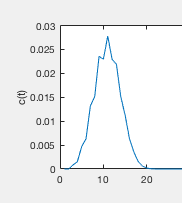
\includegraphics[scale=1]{d05}
	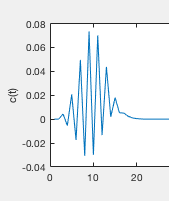
\includegraphics[scale=1]{d06}
\end{enumerate}

It is clearly visible that this model has tendencies for being numerically unstable and careful parameters choice is very important.

\subsection{Mass conservation law}
Mass conservation law states that, for closed system to all transfers of matter and energy, the mass of the system must remain constant over time. To assert, that this holds, matlab script can be expanded with vector of integrals of amount of tracer in river over time. \\

\begin{lstlisting}[language=Matlab,frame=single,label={lst:autocorr},breaklines=true,caption={Matlab script for explicit taylor method}]
...
sums = [];
% calculate in real time
for i = 1:nt
    for j = 3:(len/dx)-1
        c(i+1, j) = c(i, j) + ...
            (Cd*(1-Ca) - (Ca/6)*(Ca^2 - 3*Ca + 2))*c(i,j+1) - ...
            (Cd*(2 - 3*Ca) - (Ca/2)*(Ca^2 - 2*Ca - 1))*c(i,j) + ...
            (Cd*(1 - 3*Ca) - (Ca/2)*(Ca^2 - Ca - 2))*c(i,j-1) + ...
            (Cd*Ca + (Ca/6)*(Ca^2 - 1))*c(i,j-2);
    end
	sums(i) = sum(c(i,:));
    ...
end

K>> length(unique(sums))

ans =

   1
\end{lstlisting}
Which means, that all integrals stored in "sums" vector has same value (or roughly the same).

\section{Conclusion}
This report covered simplified simulation of river pollution using quickest Taylor model implementation. It proved its easiness to implement, and good accuracy in numerical approach to this problem, which was confirmed by mass conservation law. However, it is highly vulnerable to osculations and instability with unwise parameters choosing. All in all, author of this report is satisfied with obtained results.
\end{document}
